\section{A modeling specification for recursive organization improvement}
\label{sec:spec}
\subsection{State, improvement procedure, and change boundary}
An instance declares a task population, environment process, outcome criterion, and assessment horizon. The environment generates tasks and outcomes; actor policies receive only the observations assigned to them. At event index $t$, define
\begin{equation}
\Org_t=(X_t,D_t,L_t,\Phi_t,\Pi_t,M_t),\qquad U_t=(g_t,a_t,e_t,s_t,r_t).
\label{eq:state}
\end{equation}
The organization state $\Org$ describes who does the work and what they can know or change. The procedure $U$ describes how the team proposes, tests, selects, and retains changes. Table~\ref{tab:notation} maps their components to the PR example. Actors also have task-specific capability profiles; approval rights are recorded separately.

\begin{table}[htbp]
\caption{Core notation, illustrated by PR review routing.}
\label{tab:notation}\small
\begin{tabularx}{\linewidth}{@{}p{.15\linewidth}YY@{}}\toprule
Symbol & Meaning & PR example \\\midrule
$X$ & Actors, roles, tasks, versioned artifacts & Reviewer, agent, PR, test report. \\
$D$ & Task and resource dependencies & Approval depends on tests and reviewer availability. \\
$L$ & Decision rights & Maintainer may change routing; review board may change auditing. \\
$\Phi$ & Observation availability & Which test results or private assessments each actor can see. \\
$\Pi$ & Interaction and allocation protocols & Assignment order, review sequence, and workload allocation. \\
$M$ & Retained evidence and versions & Audit labels, trial scores, and the adopted routing rule. \\
$U=(g,a,e,s,r)$ & Generate, acquire, evaluate, select, retain & Propose a rule; audit PRs; score and select it; monitor continued use. \\
$\mathcal B$ & Declared change boundary & Routing and auditing may change; outcome criterion stays fixed. \\
$\Hist_{i,t}$ & Evidence visible to actor $i$ before event $t$ & Reports available before approval. \\
$p,\Trace,H$ & Change contract, event trace, evaluation horizon & Recorded routing change and its follow-up period. \\\bottomrule
\end{tabularx}\end{table}

\begin{definition}[Declared boundary]
A boundary $\mathcal B$ partitions fields into operational arrangements, improvement-procedure fields, and externally fixed fields for a stated comparison. It identifies authorized editors, the evaluation horizon, and the outcome criterion.
\end{definition}
An execution event changes work artifacts. An operational adaptation changes an arrangement under the declared improvement procedure. A procedure revision changes a field of $U$ and evaluates its consequences for subsequent organizational changes or outcomes. For instance, assigning a PR to a reviewer is execution; replacing its routing rule is operational adaptation; replacing the sampling program used to evaluate routing changes is procedure revision. A fixed outer selector may govern all three. The recursive designation identifies a change target relative to $\mathcal B$, not a representation-independent property of software.

This boundary also resolves overlapping implementations. $\Phi$ applies the current visibility rules, while $a$ requests evidence for a change evaluation. If one patch affects both, the implementation records the coupled fields and charges its costs once. If the outcome criterion changes, its version changes too; comparisons under the old and new criteria are reported separately.

\subsection{Events and actor-visible histories}
For the PR team, an event may be a reviewer assignment, a private assessment, or a revealed test report. An event $z$ records an identifier, logical order, actor, action, input/output artifact versions, recipients, resource use, and organization version. Actions include assignment, commitment, reveal, critique, test, escalation, approval, and patch application. Logical order represents dependency; physical timestamps can additionally represent concurrency and elapsed time.

Let $\Hist_{i,t}$ contain actor $i$'s permitted initial information and artifacts revealed to that actor before event $t$. A policy satisfies
\begin{equation}
b_{i,t}\sim\pi_i(\cdot\mid\Hist_{i,t},\Org^{\mathrm{vis}}_{i,t}),
\label{eq:information}
\end{equation}
where $\Org^{\mathrm{vis}}_{i,t}$ is the actor-visible projection of the organization state. Thus a simulator can score a decision using a hidden true error rate while the decision maker receives sampled labels only. A seed supports reproducibility without granting actors access to each other's random choices.

The ordering of commitment and reveal events represents human-first, agent-first, and parallel assessment. Parallel commitments preserve the opportunity for private judgments, while shared training data, common tools, or correlated task difficulty can still induce dependent errors. Statistical dependence is a joint property requiring measurements or explicit assumptions; it cannot be inferred from separate model names. Likewise, a public review record establishes that a review was published, not that another actor read it before deciding.

\subsection{Change contracts and retention}
A proposed routing change carries a contract: a record linking the change to its evidence, comparator, cost, and follow-up rule. Formally,
\begin{equation}
p=(\tau,v,\delta,\mathcal E,\mathcal C,c_p,H,\mathcal R_p).
\label{eq:patch}
\end{equation}
$\tau$ identifies the target and proposer; $v$ is the required input version; $\delta$ is the transformation; $\mathcal E$ identifies available evidence and its provenance; $\mathcal C$ states the comparator, population, and criterion; $c_p$ specifies resource accounting; $H$ is the horizon; and $\mathcal R_p$ specifies retention, monitoring, and rollback conditions. Contract fields may refer to separately stored artifacts. Their relationships, summarized in \cref{tab:obligations}, determine whether a comparison can be reconstructed.

\begin{table}[t]
\caption{Specification obligations and observable failure conditions. Unknown information is distinguished from a violated condition.}
\label{tab:obligations}\small
\begin{tabularx}{\linewidth}{@{}p{.19\linewidth}YY@{}}\toprule
Relation & Required condition & Failure or missing record \\\midrule
Actor--evidence & Each decision input was available to its actor beforehand. & Hidden/future input; unknown exposure history. \\
Patch--state & The target version exists and matches the expected version. & Stale patch; unversioned configuration. \\
Actor--target & The actor holds the applicable editing right at that version. & Unauthorized change; unknown historical permission. \\
Evidence--population & Sampling scope and label source support the stated population. & Uncovered stratum; unknown inclusion mechanism. \\
Outcome--criterion & Both arms use the declared criterion and horizon. & Changed success definition; censored follow-up. \\
Cost--resource & Search, outputs, labels, and transitions enter one ledger. & Omitted counterfactual output; duplicate charge. \\
Decision--memory & Accepted and rejected proposals retain evidence and versions. & Retained policy without its validation domain. \\\bottomrule
\end{tabularx}
\end{table}

Admission checks authorization, versions, available evidence, prerequisites, and resources. Efficacy is a subsequent outcome comparison. These predicates have different witnesses: permission records can justify admitting a trial, while a trial's results can justify retaining its policy. Rejected and unsuccessful revisions remain in memory because they consume resources and influence future search.

For external criterion $J$ and specified comparator $0$, the effect of a patch is
\begin{equation}
\Delta_H(p)=\E[J(\Trace_{t:t+H}^{p})-J(\Trace_{t:t+H}^{0})]-C_H(p).
\label{eq:value}
\end{equation}
$C_H$ contains costs not already included in $J$. Randomized comparisons, controlled simulation, or explicit causal assumptions are needed to estimate the two potential outcomes. Outcomes without defensible common units remain a vector with declared constraints. In the simulations below, the net-value criteria incorporate every modeled resource cost, so no additional cost is subtracted in \cref{eq:value}.

\Cref{fig:framework} connects execution to this revision loop. A software team might first change review routing, then discover that its evaluations cover only human-reviewed PRs. A second patch can alter evidence acquisition to include routine changes. That second patch is evaluated through later routing decisions and their outcomes; the mere act of adding an audit does not establish its net benefit.
\begin{figure}[!htbp]
\centering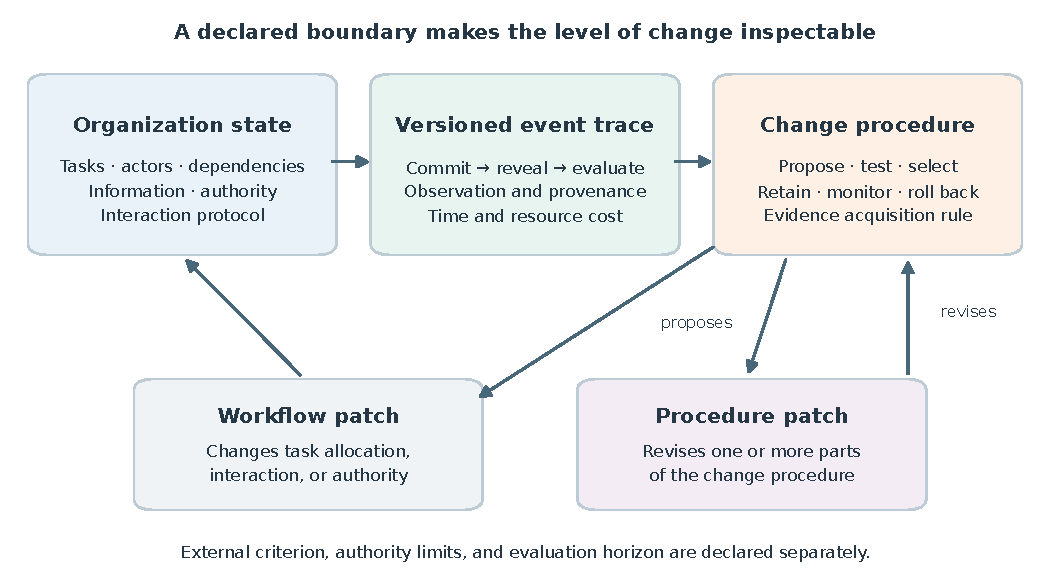
\includegraphics[width=.97\linewidth]{figures/fig1_framework.pdf}
\caption{The modeling specification connects organization state, event histories, and improvement procedures. A revision names its target, evidence, authority, and external evaluation criterion.}
\label{fig:framework}
\end{figure}
\FloatBarrier

\subsection{Organizational memory as a testable design choice}
The memory field $M$ separates three retained objects: workflow evidence, evaluation-program evidence, and adopted arrangements. Keeping a program name without its supporting observations preserves a decision but does not accumulate statistical knowledge. Keeping observations indefinitely can preserve knowledge about a population that no longer exists. An instance therefore records evidence provenance, applicability, and expiry alongside the retained policy.

The retention component $U.r$ specifies when evidence or arrangements are reconsidered. A fixed window is one such rule; changing the rule is a procedure revision at the declared boundary. In Study 1, memory rules are experimentally assigned and held fixed within a run. Evaluation programs may then change inside each memory condition. This factorial construction separates a design intervention on retention from the execution of a program-selection procedure.

Evidence generated during organizational search can serve more than one decision. A rejected program trial may still produce valid labels about a workflow. The trace records the labels once and reveals them to the permitted downstream evaluator; their cost is charged once. Comparing a policy that reuses those labels with one that discards them tests an information-transfer rule. Comparing two policies with the same trials and label reuse, while allowing only one to replace its program, tests a more specific contribution of program revision.

\subsection{What the implementation checks}
The reference implementation provides a finite checker for unique event/artifact identifiers, visible inputs, version matching, protected criteria, target-specific permissions, and patch budgets. Constructed fixtures accept a valid trace and patch and reject a hidden input and five invalid patch variants. A separate target test allows a release owner to change routing but rejects the same actor's audit-rule change; granting the review board that right admits it. This checks the operational consequences of the declared boundary.

Study 1 instantiates a narrower executable subset: retained label statistics, retained trial scores, program versions, authorized patch application, label budgets, and a modeled cost ledger. It exports trajectory outcomes, program proportions, conditional block outcomes, and example version transitions. Full implementations would additionally need to enforce all relationships in \cref{tab:obligations}, including criterion and retention contracts. The supplied checks establish conformance to their implemented predicates; the simulation studies supply evidence about efficacy within their specified settings.

Study 2 instantiates parts of Actor--evidence through purchased private and exposed judgments, Cost--resource through acquisition, production, and switching charges, and Decision--memory through retained observation counts and recorded arrangement choices. Arrangements are selected directly from a fixed catalog; they are not submitted as versioned patches to the reference checker.

Mapping public repository records supplies a complementary feasibility check. Three merged Flask PRs yield four commit artifacts and 56 mapped events: eight reviews, 42 head-commit check runs, and six opening/merge records. Artifact identifiers and recorded actions are recoverable. Historical authority, actual message exposure, effort, organization versions, and AI involvement remain unknown. Appendix~\ref{app:records} specifies the snapshot and mapping. Such a trace can expose instrumentation gaps before a team attempts a workflow-effect estimate.
